 \documentclass[a4paper,11pt]{article}
 \usepackage{graphicx}
 \usepackage[utf8]{inputenc}
 \usepackage[T1]{fontenc}
 \begin{document}
\begin{center}
	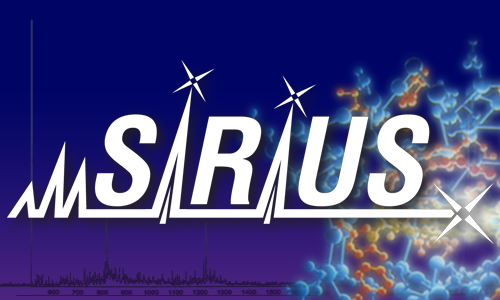
\includegraphics[width=0.9\linewidth]{sirius.png}
	Sirius 3.1
\end{center}
 
 \tableofcontents
 
 \newpage
  
 \section{Installation}
 
SI
 
 \section{Getting started.}
 
 TODO Bild vom Hauptfenster, Buttons hervorheben, Kurzbeschreibung fuer jeden Button. Für die Funktion der meisten Buttons sollte das ausreichen
 
 M1 Import experiment
 M2 Batch import
 M3 Edit
 M4 Close
 
 M5 Open workspace
 M6 Close workspace
 M7 Compute 
 
 \subsection{Data import}
 
 The Sirius GUI offers two types of data import, ''import experiment'' (M1) and ''batch impor'' (M2). 
 With ''import experiment'' it is possible to combine  several files to one experiment. 
 ''Batch import'' serves to import several experiments in a fast way while every file is assigned to one experiment. 
 Drag and Drop is supported for both operations.
 
 \subsubsection{Import experiment}
 
 This dialog is used to combine one or more files to one experiment. Adding spectra to the experiment is done via 
 the ''+'' Button or Drag and Drop. It is important for each spectra that the correct ms mode is set.  
 Only one MS1 spectrum is allowed per experiment. If multiple MS1 spectra should be used, the spectra must be merged externally.  
 The compound name and collision energies are optional and have no effect on the algorithm. 
 Both are used  for a better distinction of experiments and spectra. 
 
 \subsubsection{Batch import}
 
 The batch import is used to import several experiments at once. For this, every file is assigned to one experiment. 
 Compound name, ms levels and collision energies are taken from input files. Wrong values can be changed afterwards with the edit dialog (M3).  
 Since CSVs do not contain the necessary information, they are not supported in this mode.
 
 \subsection{Computation of molecular formulas and fragmentation trees}
 
 The computation of the molecular formulas and fragmentation trees is controlled over the compute all dialog (M7).
 This dialog computed all experiments in the workspace. Information about rare elements and instrument settings are needed.
 The focused mass is selected automatically (TODO: Wir sollten in der subsubsection schreiben nach welchen Regeln die FM gewählt wird?!)
 Furthermore, it is possible to compute a selected experiment by using the compute option in the context menu.
 This option should be used if the user wants to adapt the used focused mass or if the selected experiment differs from the other experiments in
 the workspace in terms of rare elements or instrument settings.
 
 \subsubsection{Focused mass}
 
 The focused mass must be as accurate as possible. Ideally it is equal to the mass of the monoisotopic peak of the compound. Per default, 
 the mass of the most intensive ms1 peak is used. The related textfield has an auto-completion that proposes appropriate peak masses. 
 If a MS1 spectrum is present, the corresponding masses are shown or the masses of the MS2 spectra in the other case.  
 If present the focused mass value of the input data is given as an alternative.  Often this value is not accurate. 
 But it is useful to find the correct peak mass if the most intensive peak is far away from the monoisotopic peak.
 
 \subsubsection{Rare elements}
 
 Per default the algorithms considers the common elements carbon (C), hydrogen (H), nitrogen (N), oxygen (O), phosphorus (P) and sulfur (S). 
 If it is assumed that the compound contains other rare elements, this elements should be added. To considered wrong elements will not lead necessarily 
 to wrong results. But they will increase the size of the search space, which will increase the running time and can lead to in some cases 
 to wrong molecular formulas that explain the data better than the real molecular formula.
 
 \subsubsection{Instrument settings}
 
 The Sirius algorithm uses several profiles depending on the used instrument. 
 Therefore, the used must select the correct ionization, instrument type  and mass accuracy in ppm.
 
 \subsection{Visualization of results}
 
 %TODO Bild von Ergebnispanel einfuegen, MF List und beide tabs hervorheben + Kurzerklaerung
 
 The molecular formula list contains the best molecular formulas, sorted by score. For every molecular formula, 
 the corresponding fragmentation tree is visualized in the „tree view“ tab. Alternatively, the „spectra view“ 
 tab visualizes which peak is assigned to a fragment.
 
 \subsubsection{Tree view}
 
 The tree view serves for the visualization of fragmentation trees. 
 The user has the choice between different node styles and  color schemes. 
 The shown tree can be exported as JPEG, GIF,  and PNG. 
 Alternatively, the Dot file format contains only a description of the tree. 
 It can be used to render the tree externally. The command-line tool Graphviz can 
 transform dot files into image formats (PDF, SVG, PNG etc).
 
 \end{document}
